\documentclass[a4paper, 12pt] {article}
\usepackage[spanish] {babel}
\usepackage[utf8] {inputenc}
\usepackage[T1] {fontenc}
\usepackage{bm}
\usepackage{graphicx}
\usepackage{amsmath, amsfonts, latexsym, color, textcomp, anysize}
\usepackage{float}
\renewcommand{\baselinestretch}{1}

\marginsize{1.5cm}{1cm}{1.5cm}{1.5cm}
\parindent=2mm
\parskip=3mm

\title{}
\author{Luis Basanta Pérez}
\date{}

\begin{document}
\maketitle

Al ejecutar el programa por primera vez obtuve un salto en la energía total de $0.8$. Para corregir ese salto hacemos que el sistema avance unos 5000 pasos y luego llamamos a una subrutina que vuelve a rescalar las velocidades y calculamos las energías con estas nuevas velocidades.

La gráfica que se obtiene al avanzar 500000 pasos una vez corregido el salto de energía es:

\begin{figure}[H]
\centering
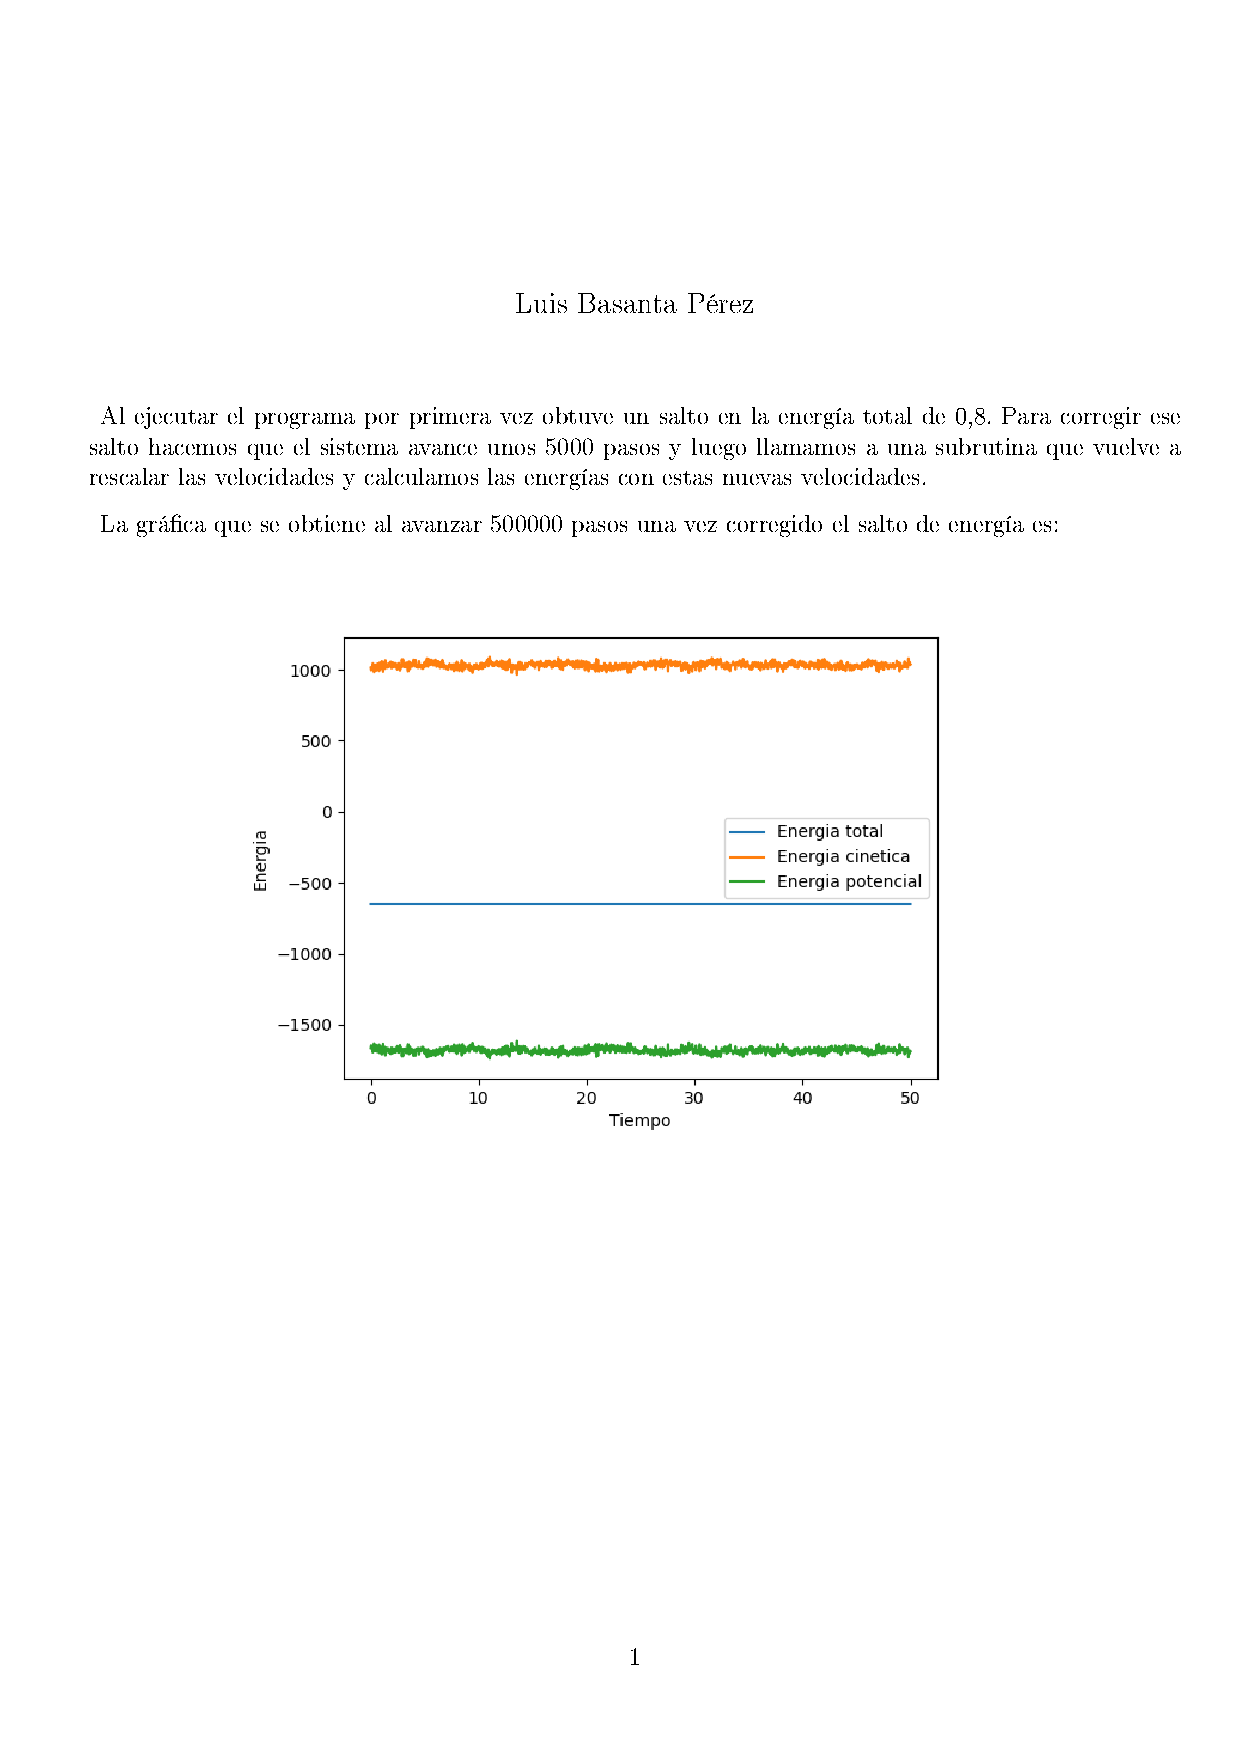
\includegraphics[width=0.7\linewidth]{Grafica energia}
\label{dibujo}
\end{figure}

\end{document}